%%%%%%%%%%%%%%%%%%%%%%%%%%%%%%%%%%%%%%%%%
% Beamer Presentation
% LaTeX Template
% Version 1.0 (10/11/12)
%
% This template has been downloaded from:
% http://www.LaTeXTemplates.com
%
% License:
% CC BY-NC-SA 3.0 (http://creativecommons.org/licenses/by-nc-sa/3.0/)
%
%%%%%%%%%%%%%%%%%%%%%%%%%%%%%%%%%%%%%%%%%

%----------------------------------------------------------------------------------------
%	PACKAGES AND THEMES
%----------------------------------------------------------------------------------------

\documentclass{beamer}

\mode<presentation> {

\useoutertheme{acis}

%Uncomment this to have the table of contents shown before each new section

%\AtBeginSection[]
%{
  %\begin{frame}
    %\frametitle{Table of Contents}
    %\tableofcontents[currentsection,currentsubsection]
    %\addtocounter{framenumber}{-1}
  %\end{frame}
%}

%Uncomment this to have the table of contents shown before each new subsection

%\AtBeginSubsection[]
%{
  %\begin{frame}
    %\frametitle{Table of Contents}
    %\tableofcontents[currentsection,currentsubsection]
    %\addtocounter{framenumber}{-1}
  %\end{frame}
%}

%Uncomment this to have the table of contents shown before each new subsubsection

%\AtBeginSubsubsection[]
%{
  %\begin{frame}
    %\frametitle{Table of Contents}
    %\tableofcontents[currentsection,currentsubsection, currentsubsubsection]
    %\addtocounter{framenumber}{-1}
  %\end{frame}
%}
}

\usepackage{graphicx} % Allows including images
\usepackage{booktabs} % Allows the use of \toprule, \midrule and \bottomrule in tables
\usepackage[T1]{fontenc}    % Makes all text copyable
\usepackage{lmodern}        % Use modern T1 font rendering
\usepackage[utf8]{inputenc} % Allows inpit in utf8
\usepackage{xcolor}
\usepackage{verbatim}


%----------------------------------------------------------------------------------------
%	TITLE PAGE
%----------------------------------------------------------------------------------------

\title[\center{Knowledge Graphs Seminar \mbox{WS 2018/19}}]{Clustering Knowledge Graphs} % The short title appears at the bottom of every slide, the full title is only on the title page
\subtitle{Knowledge Graphs Seminar WS 2018/19}

\author{Lina Molinas Comet} % Your name
\institute[RWTH Aachen] % Your institution as it will appear on the bottom of every slide, may be shorthand to save space
{
RWTH Aachen University, Germany \\ % Your institution for the title page
\medskip
\textit{lina.molinas.comet@rwth-aachen.de} % Your email address
}
\date{\today} % Date, can be changed to a custom date

\begin{document}

\begin{frame}
\titlepage % Print the title page as the first slide
\end{frame}

\begin{frame}
\frametitle{Overview} % Table of contents slide, comment this block out to remove it
\tableofcontents % Throughout your presentation, if you choose to use \section{} and \subsection{} commands, these will automatically be printed on this slide as an overview of your presentation
\end{frame}

%----------------------------------------------------------------------------------------
%	PRESENTATION SLIDES
%----------------------------------------------------------------------------------------

%------------------------------------------------
\section{Motivation} % Sections can be created in order to organize your presentation into discrete blocks, all sections and subsections are automatically printed in the table of contents as an overview of the talk
%------------------------------------------------

\section{Background and Concepts} % A subsection can be created just before a set of slides with a common theme to further break down your presentation into chunks
\subsection{Graphs}
\subsection{Knowledge Graphs}
\subsection{Knowledge-based Systems}
\subsection{Clustering}
\subsection{Other Terms}
\subsection{}

\section{State of the Art}
\subsection{General Techniques for Knowledge Graph Clustering}
\subsection{Techniques and Algorithms}
\subsubsection{Graph clustering for content aggregation for an Ontology-Based P2PKM}
\subsubsection{Structural similarity clustering entities}
\subsubsection{Entity Clustering using link features}

\section{Analysis and comparison of presented approaches}
\section{Discussion}
\section{Conclusion}



\begin{frame}
\frametitle{Motivation}
\begin{itemize}
   \item Importance of Clustering
   \item What are the common problems in the most "traditional" clustering algorithms?
   \item What are the new techniques and tool to help improve Knowledge Graph Clustering

\end{itemize}

\end{frame}

%------------------------------------------------

\begin{frame}
\frametitle{Background}

\textcolor{RWTHblue}{What are Knowlege Graphs?}


\begin{figure}[h!]
  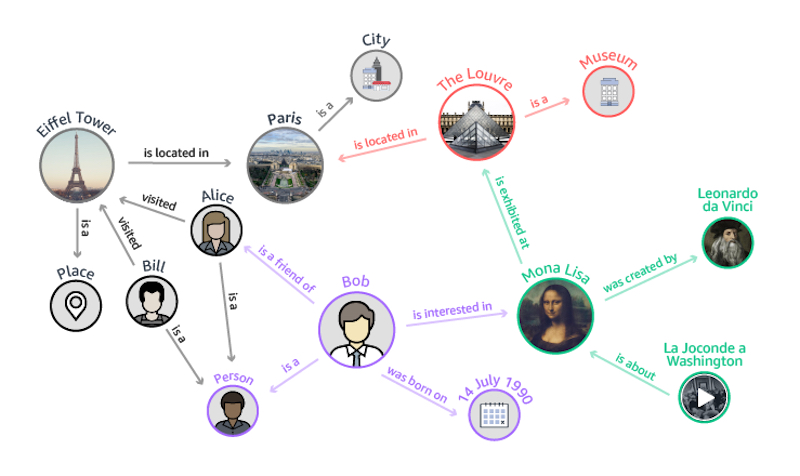
\includegraphics[width=1 \linewidth]{Amazon-Neptune-Knowledge-Graph.jpg}
  \caption{Amazon maps out the Knowledge Graph with its Neptune database service (geomarketing.com)}
\end{figure}

\end{frame}


%------------------------------------------------
\begin{frame}
\frametitle{State of the Art}
\begin{center}
 \Large{\textcolor{RWTHblue}{General Techniques}}
\end{center}
\end{frame}

%------------------------------------------------
\begin{frame}
\frametitle{State of the Art}
\begin{center}
 \Large{\textcolor{RWTHblue}{Entity Clustering using link features}}
 \begin{figure}[h!]
  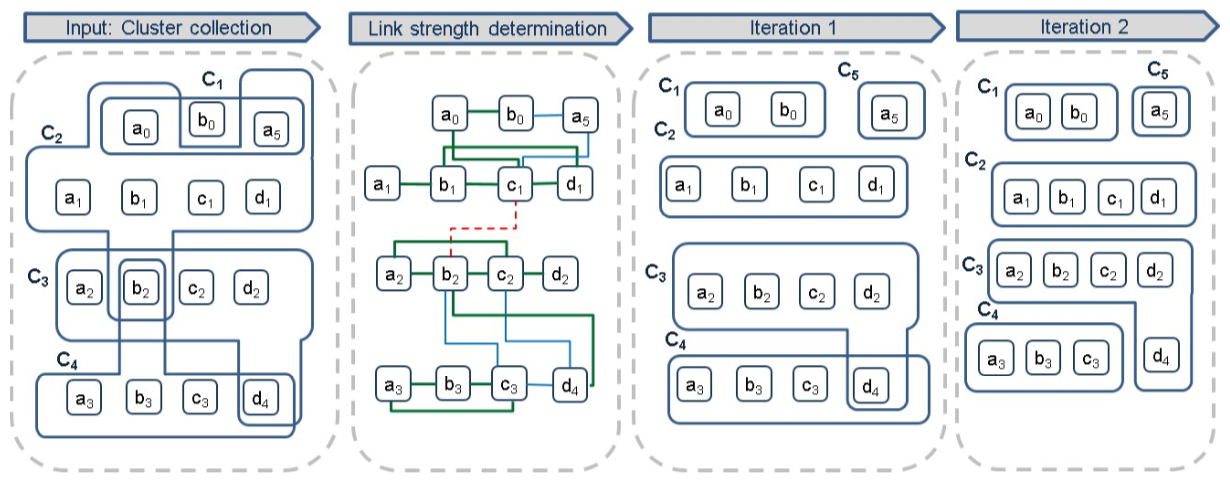
\includegraphics[width=1 \linewidth]{clip_overlap_resolution.png}
  \caption{Overlapping resolution CLIP)}
\end{figure}
\end{center}
\end{frame}

%------------------------------------------------
\begin{frame}
\frametitle{State of the Art}
\begin{center}
 \Large{\textcolor{RWTHblue}{Structural similarity clustering entities}}
 \begin{figure}[h!]
  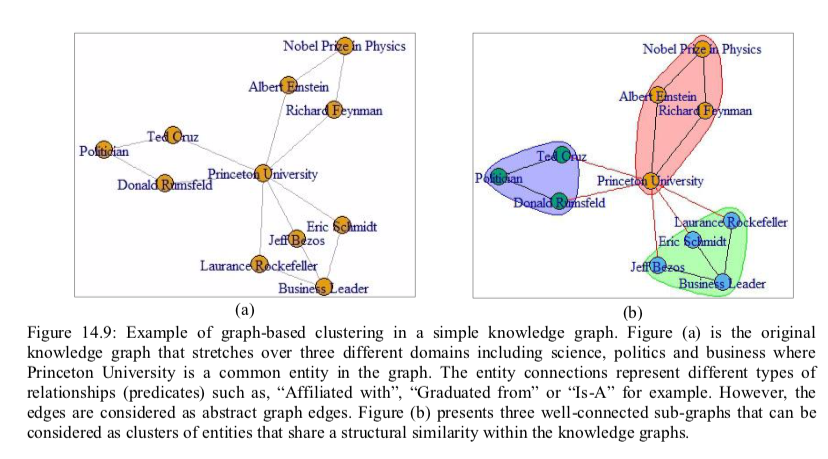
\includegraphics[width=1 \linewidth]{ex.png}
  
\end{figure}
\end{center}
\end{frame}

%------------------------------------------------

\begin{frame}
\frametitle{References}
\footnotesize{
\begin{thebibliography}{99} % Beamer does not support BibTeX so references must be inserted manually as below

\bibitem[Schmitz]{Schmitz} Schmitz, C., Hotho, A., J{\"a}schke, R., Stumme, G. (2006) 
\newblock Content Aggregation on Knowledge Bases Using Graph Clustering.
\newblock \emph{In: Sure, Y., Domingue, J. (eds.) The Semantic Web: Research and Applications. ESWC 2006}

\bibitem[Elbattah]{Elbattah} Elbattah, M., Roushdy, M., Aref, M., M.Salem, A. (2017) 
\newblock Large-Scale Entity Clustering Based on Structural Similarity within Knowledge Graphs.
\newblock \emph{In: Arun, K., Somani, G. (eds.) Big Data Analytics: Tools and Technology for Effective Planning, Edition: 1, Chapter: 14}

\bibitem[Saeedi]{Saeedi} Saaedi, A., Peukert, E., Rahm, E.  (2018) 
\newblock Using Link Features for Entity Clustering in Knowledge Graphs.
\newblock \emph{In: Gangemi, A., Navigli, R., Vidal, M., Hitzler, P., Troncy, R., Hollink, L., Tordai, A., Alam, M. (eds.) The Semantic Web. ESWC 2018}

\bibitem[Pedrycz]{Pedrycz} Pedrycz, W.  (2005) 
\newblock Knowledge-Based Clustering: From Data to Information Granules.
\newblock \emph{In: 2nd edn. Wiley-Interscience}
\end{thebibliography}
}
\end{frame}


%------------------------------------------------

\begin{frame}
\frametitle{References}
\footnotesize{
\begin{thebibliography}{99} % Beamer does not support BibTeX so references must be inserted manually as below
\bibitem{Zhang}
Zhang, X., Lv, Y., Lin, E : Object Clustering in Linked Data using Centrality. In: Proceedings of China Conference on Knowledge Graph and Semantic Computing (CCKS2016)
on Proceedings, pp. 172--183. Publisher, Location (2016). \doi{10.1007/978-981-10-3168-7\_17}

\bibitem{Ehrlinger}
Ehrlinger, L, W{\"o}{\ss}, W.: Towards a Definition of Knowledge Graphs. In: Martin, M., Cuquet M., Folmer, E. (eds.) In Joint Proceedings of the Posters and Demos Track of the 12th International Conference on Semantic Systems - SEMANTiCS2016 and the 1st International Workshop on Semantic Change \& Evolving Semantics (SuCCESS'16), CEUR-WS, vol. 1695, Leipzig, Germany (2016). \doi{10.10007/1234567890}

\bibitem{Paulheim}
Paulheim, H.: Knowledge Graph Refinement: A Survey of Approaches and Evaluation Methods. Semantic Web Journal, 489--508 (2017). \doi{10.3233/SW-160218}

\bibitem{Farber}
F{\"a}rber, M., Bartscherer, F, Menne,C., Rettinger, A.: Linked data quality of DBpedia, Freebase, OpenCyc, Wikidata, and YAGO. Semantic Web Journal, 77--129 (2018). \doi{10.3233/SW-170275}


\end{thebibliography}
}
\end{frame}

%------------------------------------------------

\begin{frame}
\frametitle{References}
\footnotesize{
\begin{thebibliography}{99} % Beamer does not support BibTeX so references must be inserted manually as below
\bibitem{Tripathi}
Tripathi, K.: A Review on Knowledge-based Expert System: Concept and Architecture. IJCA Special Issue on Artificial Intelligence Techniques-Novel Approaches \& Practical Applications (2011). \doi{10.5120/2845-226}

\bibitem{Engelmore}
Engelmore R.S.  : Artificial Intelligence and Knowledge Based Systems: Origins, Methods and Opportunities for NDE. In: Thompson D.O., Chimenti D.E. (eds.) Review of Progress in Quantitative Nondestructive Evaluation. Review of Progress in Quantitative Nondestructive Evaluation, vol. 6 A., 
Springer, Boston, MA (1987). \doi{10.1007/978-1-4613-1893-4\_1}

\end{thebibliography}
}
\end{frame}




%------------------------------------------------

\begin{frame}
\Huge{\centerline{Q \& A}}
\end{frame}

%----------------------------------------------------------------------------------------


\begin{comment}

\end{comment}

\end{document} 
